\documentclass{standalone}
\usepackage{tikz}
\usetikzlibrary{arrows.meta}
\usetikzlibrary{angles}
\usepackage{siunitx}
\usepackage{unicode-math}
\setmainfont{Times New Roman}
\setmathfont{NewCMMath-Book}
\setmathfont{Times New Roman}[
  range = {up/{num, latin}}
]

\begin{document}
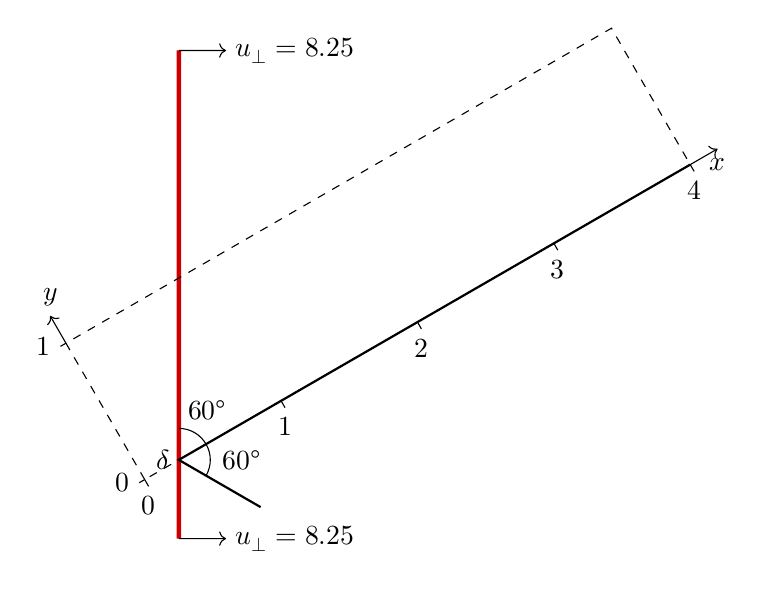
\begin{tikzpicture}[scale=2, rotate=30]
  % axes
  \draw[->] (4,0) -- +(0.2,0) node[below] {$x$};
  \draw[->] (0,1) -- +(0,.2) node[above] {$y$};
  % ticks
  \foreach \i in {0,...,4}
    \draw (\i,0) -- +(0,-.05) node[below] {$\i$};
  \foreach \i in {0,1}
    \draw (0,\i) -- +(-.04,0) node[left] {$\i$};
  % lines and nodes
  \draw[ultra thick, red!80!black] (0.25,0) coordinate (x0) -- +(60:2.6) coordinate (us);
  \draw[ultra thick, red!80!black] (x0) -- +(-120:0.5) coordinate (ut);
  \draw[dashed] (0,0) rectangle (4,1);
  \path (us) -- (x0 -| us) coordinate (xs);
  \draw[->] (us) -- +(-30:.3) node[right] {$u_\perp=8.25$};
  \draw[->] (ut) -- +(-30:.3) node[right] {$u_\perp=8.25$};
  \draw[thick] (4,0) -- (x0) -- +(-60:.6) coordinate (xt);
  \path node[left] at (x0) {$\delta$};
  % angle
  \draw pic[draw,pic text=$\ang{60}$, angle eccentricity=1.8, angle radius=.4cm] {angle=xs--x0--us};
  \draw pic[draw,pic text=$\ang{60}$, angle eccentricity=2.0, angle radius=.4cm] {angle=xt--x0--xs};
  \end{tikzpicture}
\end{document}
